\namedchapter{Rys historyczny}
\namedsection[Adam Zieliński]{Historia robotyki}
Słowo ,,robot" wywodzi się z języka czeskiego, gdzie oznacza ciężką pracę. 
Według słownika języka polskiego słowo to oznacza urządzenie zastępujące człowieka przy wykonywaniu niektórych czynności. Po raz pierwszy, w tym kontekście, zostało ono użyte w 1920 r. przez czeskiego pisarza Karela \newtie{C}apka w komedii R.U.R.(Rossum Universal Robots)\cite{Czech}. Precyzyjną definicję tego słowa przedstawiła w 1979 roku grupa \textit{Robotics Industries Association} określając robota jako: ,,Programowalny, wielofunkcyjny manipulator zaprojektowany do przenoszenia materiałów, części, narzędzi lub specjalizowanych urządzeń poprzez różne programowalne ruchy, w celu realizacji różnorodnych zadań."\cite{def_robota}.
Temat robotyki był bardzo często i szeroko poruszany przez pisarzy fantastyki naukowej, którzy w swoich dziełach wykorzystywali motyw buntu maszyn przeciwko ludzkości. Efektem tego było pojawienie się trendu filozoficznego mówiącego o etyce robotów. Jednym z twórców tego nurtu, Isaac Asimow, zaproponował kilka reguł, którymi powinna kierować się każda inteligentna maszyna\cite{prawa_robota}:
\begin{enumerate}
\item Robot nie może skrzywdzić człowieka, ani przez zaniechanie działania dopuścić, aby człowiek doznał krzywdy.
\item Robot musi być posłuszny rozkazom człowieka, chyba że stoją one w sprzeczności z Pierwszym Prawem.
\item Robot musi chronić sam siebie, jeśli tylko nie stoi to w sprzeczności z Pierwszym lub Drugim Prawem.
\end{enumerate}
Mówi się że, robotyka jest owocem wszystkich dotychczasowych osiągnięć ludzkości w każdej dziedzinie. Łączy w sobie przede wszystkim elementy : mechaniki, automatyki, elektroniki, sensoryki oraz cybernetyki.
Jej poszczególne elementy były rozwijane na przestrzeni setek a nawet tysięcy lat. Pierwsze wzmianki historyczne dotyczące budowy robotów sięgają około 350 roku p.n.e. i dotyczą greckiego matematyka Archtasa z Tarentu, który rzekomo zbudował ptaka napędzanego sprężonym powietrzem oraz potrafiącego latać. Niestety ale zweryfikowanie tej wiadomości jest bardzo skomplikowane i nie daje jednoznacznej odpowiedzi. Wskazuje ona jednak na zainteresowanie ludzkości budową maszyn-robotów, które pierwotnie miały naśladować naturę. Za początek rozwoju robotyki uważa się przełom XV oraz XVI wieku, w którym za sprawą wielkiego wynalazcy - Leonadra da Vinci powstało wiele interesujących konstrukcji. Jego projekty niejednokrotnie znacznie wykraczały poza czasy, w których żył. W swoich badaniach pozostawał wierny aforyzmowi ,,Mądrość jest
córką doświadczenia" - w związku z czym zaprojektowane przez niego konstrukcje nie opierały się na dotychczasowych teoretycznych osiągnięciach ówczesnej Europy a na własnych badaniach, pomiarach oraz próbach\cite{da_vinci}.  Na ilustracji \ref{czolg_leon} przedstawiony został szkic przedstawiający jedną z wymyślonych przez Leonarda da Vinci maszyn wojennych - przodek współczesnego czołgu, który miał miotać kamieniami w wroga oraz być napędzany siłą ludzkich mięśni.

  \begin{figure}[H]
    \begin{center}
      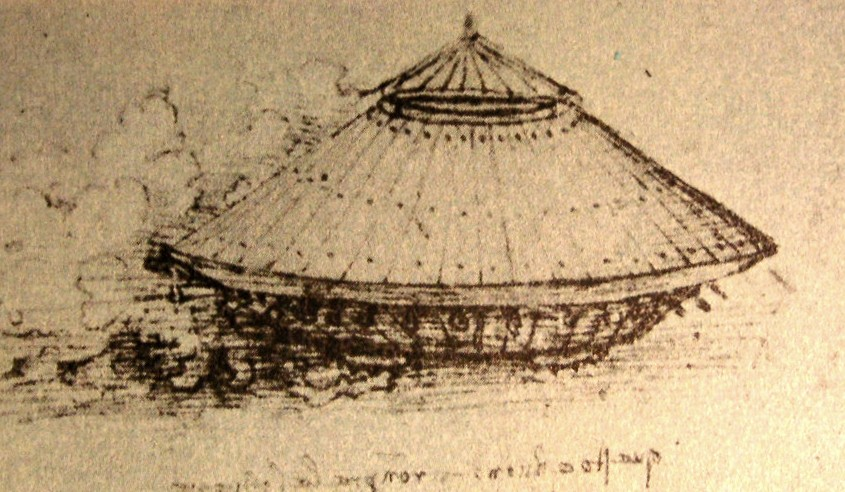
\includegraphics[scale=0.3]{imgs/Leonardo_tank.jpg}
 	\caption[Czołg Leonarda da Vinci]{\small{Szkic Leonarda da Vinci przedstawiający jego koncepcję czołgu.}\footnotemark}
	\label{czolg_leon}
    \end{center}
  \end{figure}
  \footnotetext{\emph{Czołg Leonarda da Vinci}, http://italoteka.blogspot.com,  (data dostępu 21.04.2015r.)}
Wiek XX niesie za sobą bardzo gwałtowny rozwój robotyki, który rozpoczął się w momencie skonstruowania w latach 40-tych pierwszego komputera. Ich rozwój był dodatkowo spotęgowany poprzez wybuch II wojny światowej i potrzebę łamania szyfrów dyplomatycznych.
W latach 50-tych wynaleziony został tranzystor, który aktualnie jest podstawowym elementem każdego urządzenia. Pozwolił on w znacznej mierze na zmniejszenie gabarytów komputerów (jednostek obliczeniowych), zmniejszenie zapotrzebowania na energię oraz wzrost mocy obliczeniowej co pozwoliło na konstrukcję autonomicznych robotów mobilnych.
Robotami mobilnymi nazywamy pojazdy, mogące zmieniać swoje położenie w przestrzeni. Dotyczy to nie tylko pojazdów jezdnych, ale także kroczących oraz latających. 
W 1956 r. ukończona została budowa elektrycznej wiewiórki\cite{robot_squee} (rysunek \ref{squee}), która posiadała dwa ,,zmysły": wzroku - zrealizowanego przy wykorzystaniu dwóch lamp fotoelektronowych oraz dotyku - dwóch krańcówek.  Napęd został zbudowany w oparciu o silniki elektryczne. Zwierzak, gdy zobaczył żołędzia (w tym przypadku jasno oświetlony punkt) kierował się w jego stronę, podnosił owoc przy pomocy ,,szufli" a następnie kierował się ,,do gniazda" - czyli miejsca, gdzie znajdowało się pulsacyjne źródło światła. Mimo ,iż realizowane zadanie jest bardzo proste to możemy mówić tutaj o pewnego rodzaju intelgencji ponieważ wiewiórka wykonywała pewną sekwencję ruchową bez interwencji człowieka ale w zależności od tego, co działo sie w jej otoczeniu.

  \begin{figure}[H]
    \begin{center}
      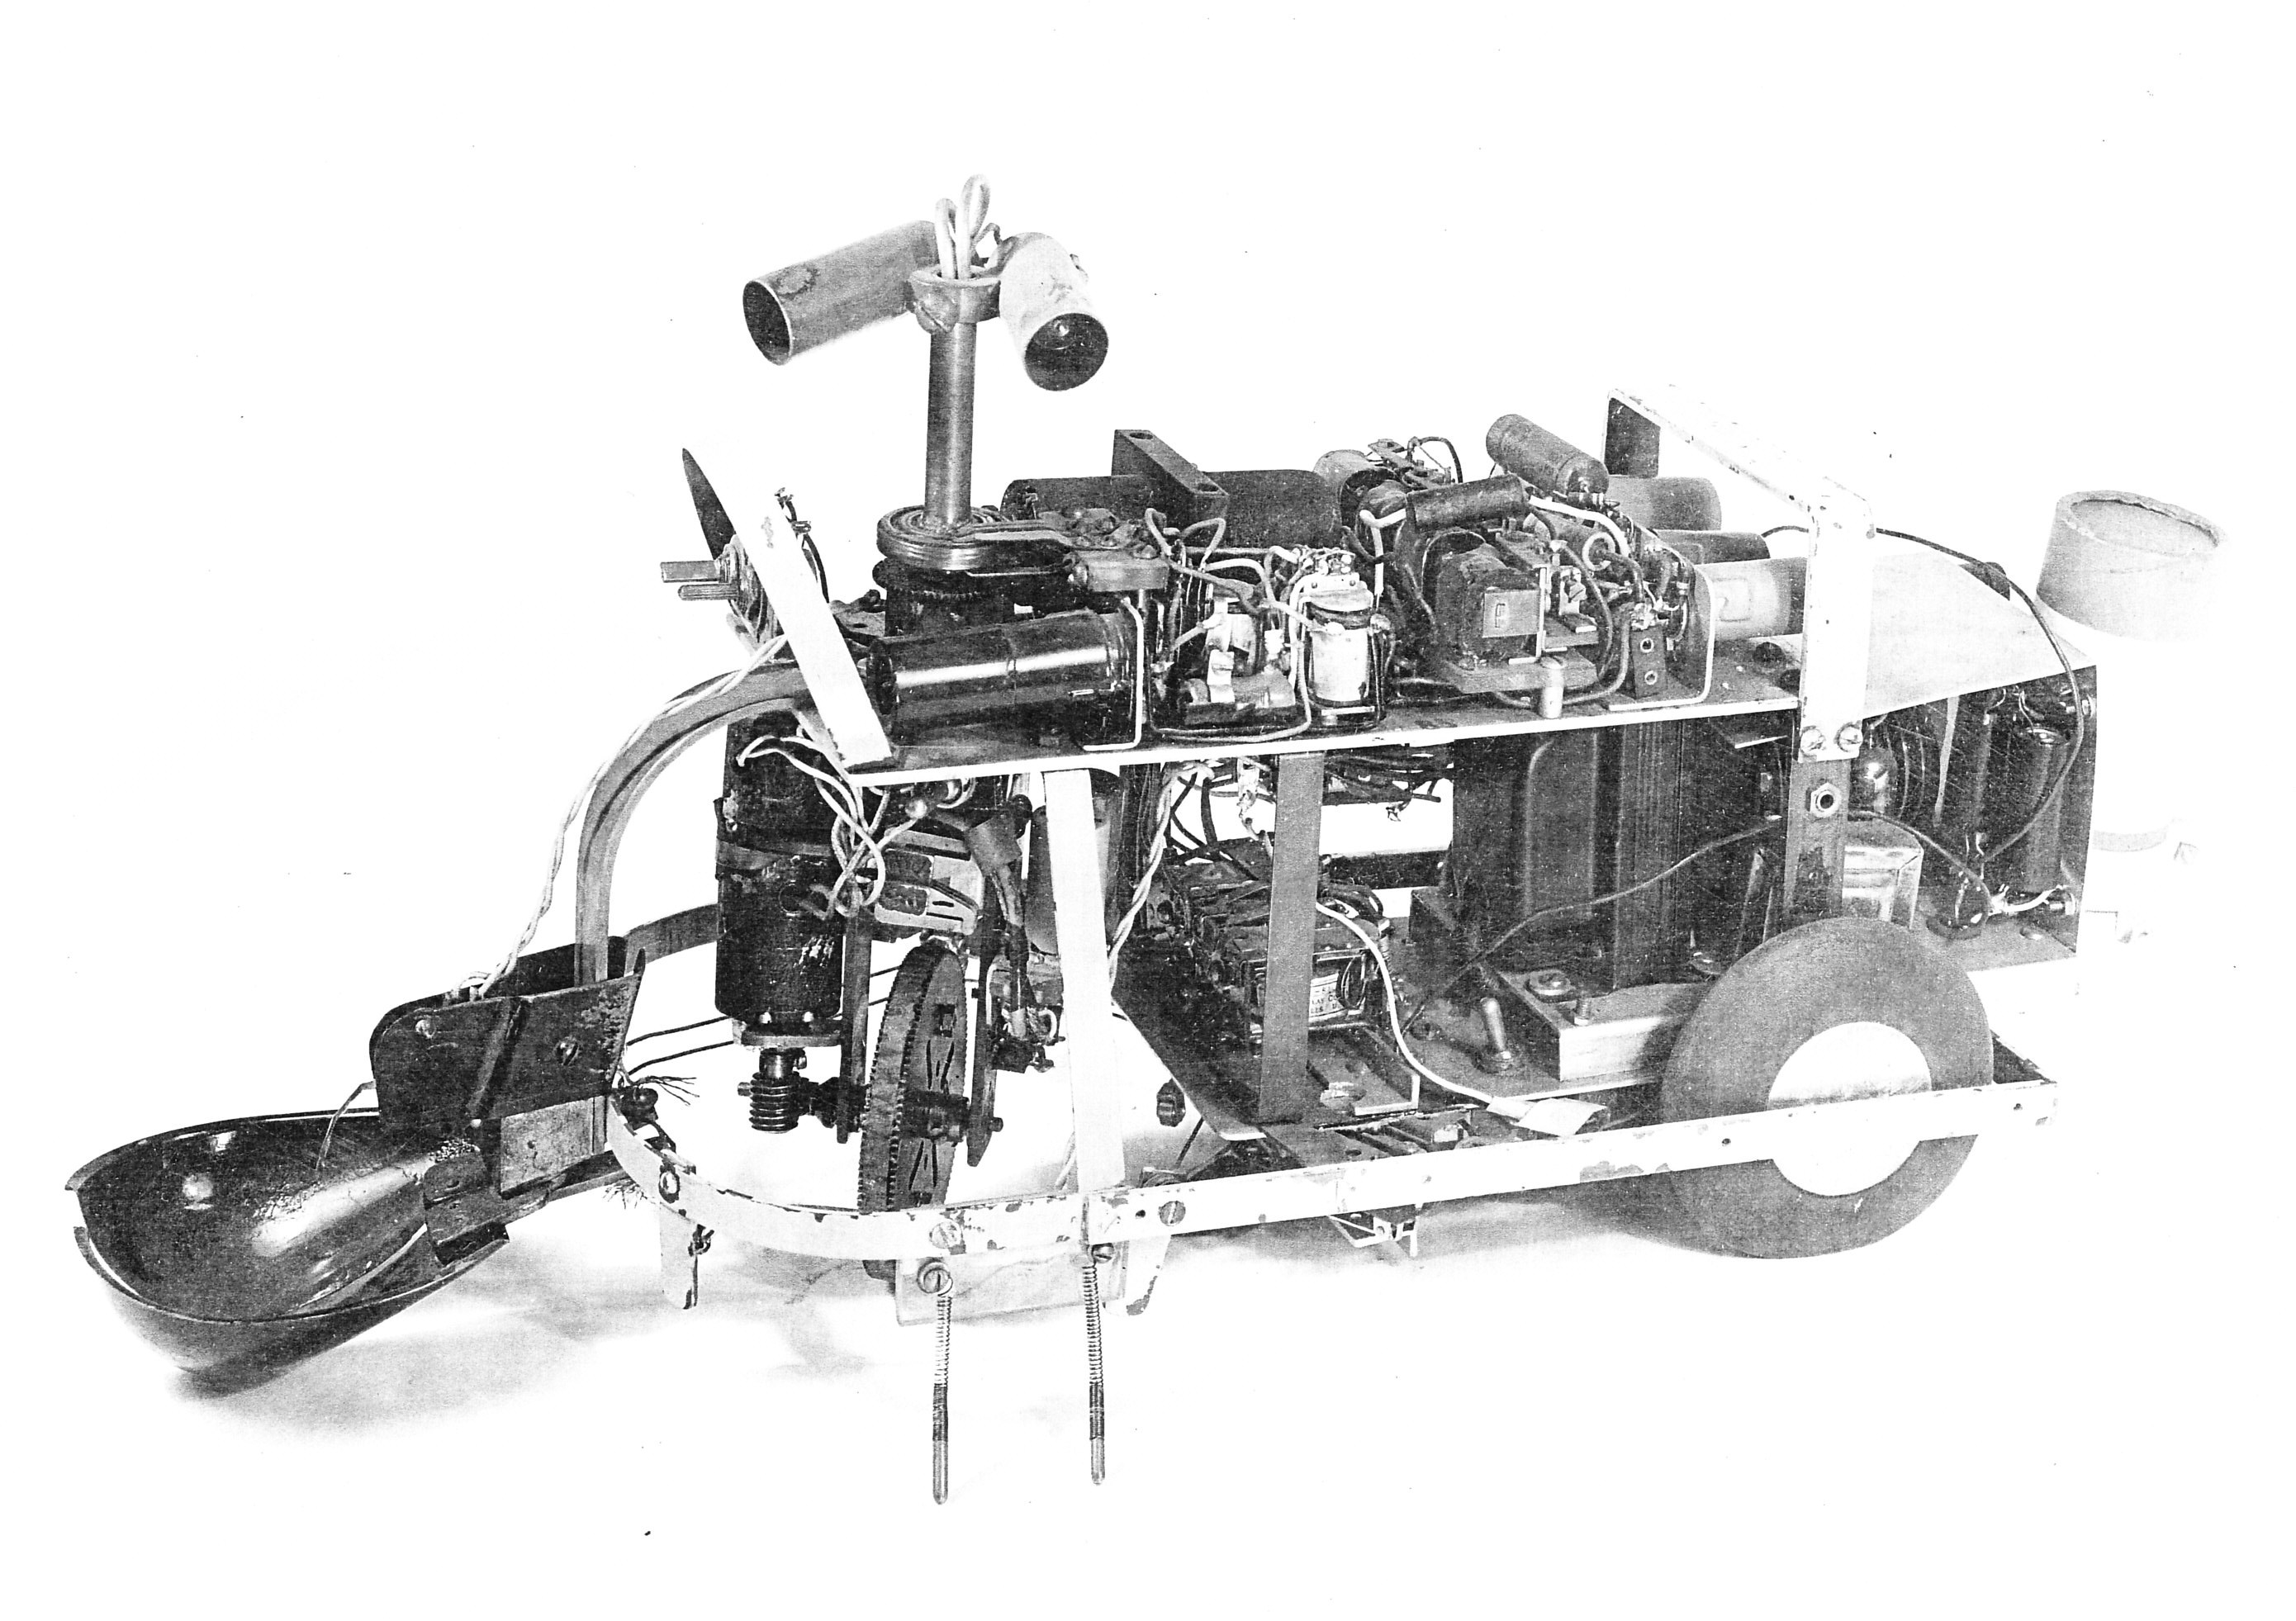
\includegraphics[scale=0.4]{imgs/Squee.jpg}
 \caption[Robot \textit{Squee}]{\small{Robot Squee zbudowany prze Jacka Koffa w 1959r.}\footnotemark}
        \label{squee}
    \end{center}
  \end{figure}
  \footnotetext{\emph{Robot Squee}, http://cyberneticzoo.com/,  (data dostępu 21.09.2015r.)}

Kolejne lata niosą za sobą coraz większą miniaturyzację wszelkich podzespów elektronicznych. Nie tylko zamykane są one w coraz mniejszych obudowach (pierwszy układ scalony - Jack St. Clair Kilby w 1958 r.) ale także charakteryzują się coraz wyższą sprawnością. Doprowadza to do tego, że pojazdy mobilne stają się obiektem zainteresowania służb specjalnych. W ten sposób w 1984 r. powstaje Prowler (rysunek \ref{state}) - pierwszy zdalnie sterowany robot o przeznaczeniu militarnym. Platforma ta mogła pełnić różne funkcje: od roli wsparcia - wyposażona w karabiny maszynowe, po funkcje rozpoznawcze - wyposażona w kamery.

  \begin{figure}[H]
    \begin{center}
      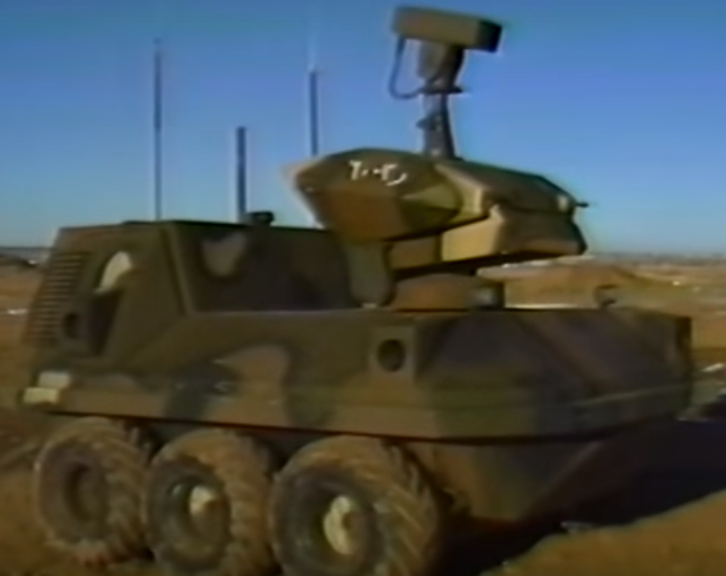
\includegraphics[scale=0.4]{imgs/state.png}
 \caption[Pojaz wojskowy \textit{Prowler}]{\small{Wojskowy robot mobilny Prowler .}\footnotemark}
        \label{state}
    \end{center}
  \end{figure}
  \footnotetext{\emph{Robot Defense Systems Prowler 1985}, https://youtube.com/,  (data dostępu 22.09.2015r.)}

Aktualnie najbardziej zaawansowanymi robotami mobilnymi są pojazdy wykorzystywane przez agencje kosmiczne do eksploracji kosmosu. Ich zaawansowana konstrukcja jest efektem bardzo rygorystycznych założeń jakie są im stawiane, tzn.: możliwie jak najmniejsze rozmiary, waga, wysoka mobilność oraz niezawodność, możliwość pracy w ciężkich, nieznanych warunkach środowiskowych. Na dodatek muszą one być zdolne do prowadzenia badań oraz zbierania próbek. Przykładem tej klasy robota może być marsjański łazik Curiosity Rover (rysunek \ref{lazik}).

  \begin{figure}[H]
    \begin{center}
      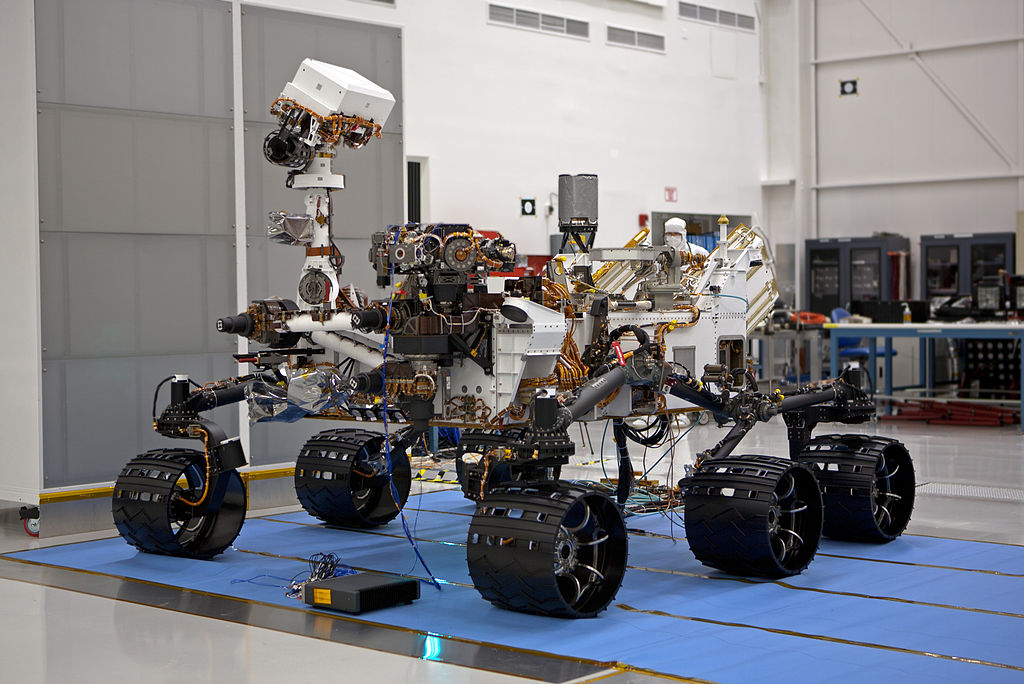
\includegraphics[scale=0.8]{imgs/curiosity.png}
 \caption[Łazik marsjański \textit{Curiosity}]{\small{Łazik marsjański Curiosity.}\footnotemark}
        \label{lazik}
    \end{center}
  \end{figure}
  \footnotetext{\emph{\textit{Curiosity}}, http://i.space.com/,  (data dostępu 22.09.2015r.)}

\namedsection[Daniel Łukwiński]{Historia czołgu}
Od zarania dziejów za wojnami krył się najszybszy oraz najgwałtowniejszy rozwój technologiczny. Rozwój cywilizacyjny następuje nieco później, ponieważ każda nowa technologia (jak np. GPS czy Internet) najpierw wprowadzana jest na potrzeby wojska a dopiero w późniejszych latach wprowadzana jest do użytku dla ludności cywilnej. Podobnie miała się sytuacja z I wojną światową - konflikt ten dał początek m.in. bojowym pojazdom opancerzonym, które otrzymały nazwę czołgów.

I wojna światowa była jednym z największych konfliktów zbrojnych w dziejach ludzkości, który walkami ogarnął niemalże całą Europę. Do jej wybuchu przyczyniła się nie tylko sytuacja polityczna ale także nastroje panujące wówczas w społeczeństwie, które ,,chciało wojny". I Wojna Światowa niewątpliwie na zawsze odmieniła pola walki. Jeszcze przed jej rozpoczęciem nastąpił intensywny rozwój broni maszynowej - jednym z pierwszych, w pełni sprawnych, karabinów maszynowych była tak zwana kartaczownica Gatlinga, skonstruowana już w 1861 roku. Jednak dopiero podczas I wojny światowej broń maszynowa rozpowszechniła się na tyle, żeby diametralnie zmienić oblicze pola walki. Linie obronne zostały gęsto obsadzone ciężkimi karabinami maszynowymi, takimi jak brytyjski Vickers czy wiele wersji karabinów Maxima, które osiągały praktyczną szybkostrzelność na poziomie 500-600 pocisków na minutę oraz zasięg przekraczający kilometr. Z kolei oddziały piechoty otrzymały broń lżejszą (np. francuski ręczny karabin maszynowy Chauchat czy brytyjski lekki karabin Lewis), która, mimo gorszych parametrów od wspomnianych wcześniej konstrukcji, była rewolucyjną zmianą na tle karabinów powtarzalnych, będących do tej pory jedyną bronią piechoty. I wojna światowa była konfliktem, w którym atakująca piechota była zasypywana zbierającym śmiertelne żniwo gradem pocisków. W efekcie tego morale żołnierzy bardzo szybko podupadło i nie chcieli oni już ginąć w imię wyższości racji politycznych. Konflikt przekształcił się w wojnę pozycyjną, w której piechota więcej czasu spędzała w okopach niż walcząc. Wszelkie znane metody walki zawodziły w tej nowej sytuacji: atak kawalerii miał jeszcze mniejsze szanse powodzenia niż piechoty, a stosowane na wielką skalę nawały artyleryjskie nie były w stanie wystarczająco zmiękczyć linii obronnych.
Aby wygrać wojnę należało w jakiś sposób dostać się bliżej przeciwnika. Już w pierwszym okresie wojny stosowano na małą skalę pojazdy opancerzone. Jednak były to pojazdy kołowe, które nie miały racji bytu poza utwardzonymi drogami. W celu przedarcia się przez ,,ziemię niczyją", czyli strefę pomiędzy okopami, skonstruowano gąsienicowy pojazd opancerzony. Co ciekawe, zadania tego podjęło się \textit{Royal Navy}, czyli marynarka wojenna Wielkiej Brytanii. Jej wpływ na projekty był silnie widoczny: pierwsze pojazdy nazywano Okrętami Lądowymi (\textit{Land Ships}), a uzbrojenie znajdowało się w sponsonach (tj. występach z boku kadłuba, służących właśnie do mocowania uzbrojenia) \cite{wojna_pancerna}. Przykładem tego typu pojazdów jest przedstawiony na ilustracji \ref{czolg_ws} Mark I, którego specjalnie uformowane gąsienice (w kształt równoległoboku) pozwalały łatwiej pokonywać zasieki wroga. Inne kraje biorące udział w walkach na froncie zachodnim szybko podchwyciły ideę opancerzonych pojazdów gąsienicowych, co zaowocowało mnogością koncepcji konstrukcyjnych i szukania, często metodą prób i błędów, najefektywniejszych rozwiązań. Przykładem zupełnie innego podejścia do konstrukcji czołu jest przedstawiony na ilustracji \ref{czolg_ft} francuski Renault FT.

  \begin{figure}[H]
    \begin{center}
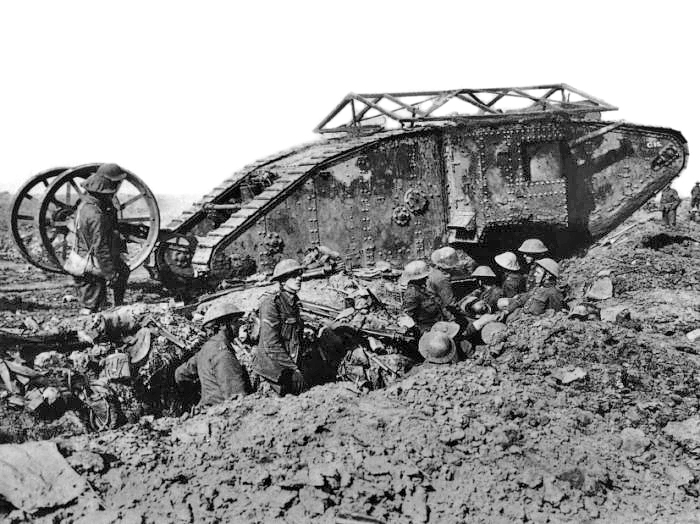
\includegraphics[scale=1.5]{imgs/ws_czolg.jpg}
 \caption[Czołg \textit{Mark I}]{\small{Czołg Mark I użyty pierwszy raz w bitwie pod Sommą w 1916 r.}\footnotemark}
        \label{czolg_ws}
    \end{center}
  \end{figure}
\footnotetext{\emph{Czołg Mark I}, http://mtg.domek.org/, (data dostępu 22.10.2015 r.)}

  \begin{figure}[H]
    \begin{center}
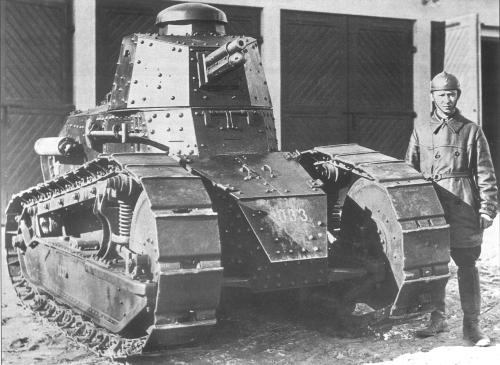
\includegraphics[scale=1.5]{imgs/ft17.jpg}
 \caption[Czołg \textit{Renault FT}]{\small{Renault FT, lekki czołg francuski z okresu I wojny światowej.}\footnotemark}
        \label{czolg_ft}
    \end{center}
  \end{figure}
\footnotetext{\emph{Czołg Renault FT}, https://pibwl.republika.pl/, (data dostępu 22.10.2015 r.)}


Wszystkie zastosowane pojazdy miały jednak podobne cele na polu walki - wspierać nacierającą piechotę, służyć dla niej jako osłona i niszczyć umocnienia przeciwnika. Ostatecznie zastosowanie czołgów pozwoliło na szybsze zakończenie I wojny światowej, jednakże początkowo większość wojskowych nie dostrzegała w tych pojazdach szerszego potencjału militarnego. Wynikało to z faktu, że czołgi w tamtym okresie były bardzo powolne i słabo opancerzone - gwałtowny rozwój techniki w tej dziedzinie miał dopiero nastąpić. Pojazdy z okresu I wojny światowej dysponowały pancerzem mogącym powstrzymać co najwyżej ogień z karabinów maszynowych (a i to nie zawsze) oraz prędkością jazdy porównywalną z tempem nacierającej piechoty. Jednak już w 1928 roku, amerykański inżynier i wynalazca Walter Christie, opatentował zawieszenie gąsienicowe oparte o duże, niezależne zawieszone koła nośne, na których rozpięte były gąsienice \cite{wojna_pancerna}. Patent ten, zakupiony m.in. przez Wielką Brytanię oraz Rosję, umożliwił budowę rodziny czołgów rozwijających prędkości przekraczające 60 km/h.

  \begin{figure}[H]
    \begin{center}
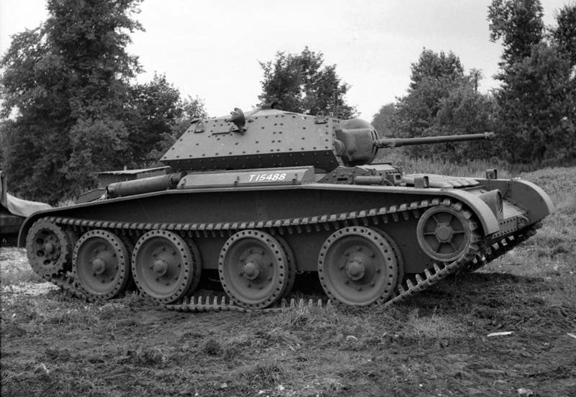
\includegraphics[scale=0.4]{imgs/covenanter.jpg}
 \caption[Czołg \textit{Cruiser Mk V ,,Covenanter"}]{\small{Brytyjski czołg Cruiser Mk V ,,Covenanter", zbudowany w oparciu o zawieszenie Christiego.}\footnotemark[7]}
        \label{covenanter}
    \end{center}
  \end{figure}
\footnotetext[7]{\emph{Czołg Cruiser Mk V}, http://worldwar2headquarters.com/, (data dostępu 12.10.2015 r.)}


Rozwój nowych systemów zawieszenia, napędu czy amortyzacji, umożliwiał tworzenie coraz bardziej mobilnych pojazdów. Rozwijała się także technika metalurgiczna, umożliwiające produkcję coraz grubszych płyt pancernych, dzięki czemu czołgi stawały się odporne na broń coraz większego kalibru. Ten rozwój pociągnął z kolei za sobą potrzebę montowania w pojazdach coraz silniejszych dział. Całość przedstawionego tutaj postępu czyniła z czołgu broń coraz bardziej kompletną i wszechstronną. Większość decydentów w armiach świata nie dostrzegało jednak potencjału tej, nowej jeszcze, broni. Jednym z wyjątków była III Rzesza, która w latach 30-tych zaczęła formować niezależne dywizje pancerne.

We wrześniu 1939 roku rozpętała się II wojna światowa, która pokazała, jak skuteczną bronią może być czołg w rękach kompetentnego dowódcy. Podczas inwazji na Francję obie strony dysponowały znacznymi siłami pancernymi, jednak mobilne i niezależne zgrupowania pancerne Wehrmachtu rozbiły rozproszone i przywiązane do piechoty czołgi francuskie. W tym momencie rozpoczął się niezwykle szybki rozwoju broni pancernej, będący wyścigiem zbrojeń pomiędzy stronami konfliktu. Wszystkie istotne parametry wozów bojowych rosły, a trafne koncepcje szybko rozprzestrzeniały się między biurami projektowymi. Koniec II wojny światowej przyniósł dużo bardziej ujednoliconą koncepcję czołgu jako uniwersalnej broni na polu bitwy. Zaowocowało to powstaniem pojęcia MBT (\textit{Main Battle Tank}), a więc czołgu podstawowego, który stał się po wojnie podstawą do tworzenia wojsk pancernych we wszystkich armiach świata, aż do dnia dzisiejszego.

MBT charakteryzuje się przede wszystkim wysoką mobilnością oraz silnym uzbrojeniem, gdyż doświadczenie pokazało, że najlepszym sposobem na przetrwanie na polu walki jest zniszczenie przeciwnika zanim ten będzie w stanie zlokalizować ciebie. W tym czasie na świecie rozpoczął się także gwałtowny rozwój elektroniki, którą zaczęto na coraz szerszą skalę stosować w sprzęcie wojskowym, m.in. w czołgach. Jednym z przykładów może być wprowadzenie systemów aktywnej noktowizji do radzieckich czołgów w latach 60-tych. Właśnie nowoczesna elektronika stała się jednym z głównych obszarów, na którym zaczęli ze sobą konkurować konstruktorzy bojowych pojazdów opancerzonych. O tym, jak wielką różnicę potrafi ona zrobić na polu walki stanowi chociażby przebieg największej bitwy pancernej w historii, która miała miejsce podczas operacji Pustynna Burza w 1991 roku. Po obu stronach konfliktu wzięło w niej udział około 8 tysięcy czołgów. Rozbudowane sytemu łączności oraz zaawansowana optyka dzienna i nocna (skutecznie wykorzystywana podczas nocnych natarć) pozwoliły zminimalizować starty własne koalicji pod dowództwem Stanów Zjednoczonych do poziomu ok. 0,4\% strat przeciwnika. Jednym z czołgów biorących udział w tej operacji był brytyjski Challenger I, przedstawiony na ilustracji \ref{challenger}.

  \begin{figure}[H]
    \begin{center}
      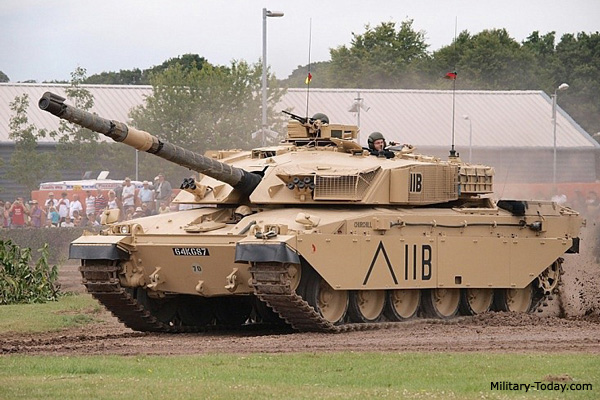
\includegraphics[scale=0.5]{imgs/chal1.jpg}
 \caption[Czołg \textit{Challenger I}]{\small{Challenger I, brytyjski czołg podstawowy (MBT).}\footnotemark[8]}
        \label{challenger}
    \end{center}
  \end{figure}
\footnotetext[8]{\emph{Czołg Challenger I}, http://military-today.com/, (data dostępu 22.10.2015 r.)}

W chwili obecnej trwają dalsze prace nad udoskonaleniem koncepcji czołgu na współczesnym polu walki. W latach 90-tych panowało przekonanie, że czasy tego rodzaju broni już przemijają, jednak ostatnie konflikty zbrojne pokazały, że wcale tak nie jest. Broń pancerna w dalszym ciągu intensywnie się rozwija, tak pod kątem koncepcji mechanicznych, jak i stosowania zaawansowanej techniki do coraz większej ilości zadań. Warte odnotowania jest m.in. dążenie do daleko idącego zredukowania ilości załogi \cite{programy_rozwoju}. Aby to umożliwić konieczne jest przejęcie części zadań załogi przez automatyczne systemy, takie jak automatyczne magazyny amunicyjne czy algorytmy służące do identyfikacji celów w polu widzenia pojazdu. Współczesna elektronika ma także zastosowanie w takich obszarach jak: maskowanie pojazdu na płaszczyźnie optycznej, termicznej oraz radiowej, wsparcie systemów wizyjnych w postaci analizy obrazu ułatwiającej jego interpretację przez załogę, rozbudowane systemy komunikacyjne na różnych poziomach dowodzenia czy złożone systemy stabilizujące ruch działa \cite{czolg_przyszlosci}.

Analizując kierunki rozwoju broni pancernej da się zauważyć ich zbieżność z tematem przedstawianej pracy inżynierskiej. Autonomiczna praca pojazdu, wyręczająca załogę z części obowiązków oraz automatyczne systemy poszukiwania oraz identyfikacji celu na podstawie danych zbieranych przez systemy wizyjne pojazdu są tematami rozwijanymi w wielu ośrodkach konstrukcyjnych zaangażowanych w rozwój systemów wojskowych.

